\documentclass{article}
\usepackage[utf8]{inputenc}
\usepackage{physics}
\usepackage{amsmath}
\usepackage{showlabels}
\usepackage{amssymb}
\renewcommand{\vec}[1]{\ensuremath{\mathbf{#1}}}
\newcommand{\uvec}[1]{\ensuremath{\hat{\mathbf{#1}}}}


\title{Statistical Computing for Scientists and Engineers\\[1em] Final Homework}
\author{Jiale Shi}
\date{Dec/10/2018}

\usepackage{natbib}
\usepackage{graphicx}
\usepackage{array}
\begin{document}
\maketitle

\newpage
\section{EM algorithm}
Implement the EM algorithm for estimating the parameters of a mixture of Gaussians with isotropic covariances using the data provided on data resources. There are two data sets each of which is two-dimensional. You can write your own or use any available code for mixture of Gaussians (e.g. you ca use the code in the code director with some changes to account for the isotropic covariances. Also see the accompanying paper Unsupervised Learning of Finite Mixture Models, M.Figueiredo and A.K. Jain.)

Experiment with the number of mixtures and comment on the trade-off between the number of mixture and goodness of fit (i.e. log-likelihood) of the data. Plot the log-likelihood as a function of the number of components of a mixture of Gaussians to support your argument.

Find a fixed number of Gaussians that works well for each data set.

Plot the estimated Gaussians as one-sigma contours of each mixing component on top of the training data.

List the mean, covariance and mixing weights of each mixture component.

\textbf{Solution}:
Implement the EM algorithm for estimating the parameters of a mixture of Gaussians with isotropic covariances. The isotropic covariances maxtrix means the covariance matrix is diagonal and all elements on the diagonal is equal.

\begin{equation}
    \textbf{C}_{\mbox{isotropic}} = \lambda \textbf{I} = \left( \begin{array}{cc}  \lambda & 0 \\ 0 & \lambda
    \end{array} \right)
\end{equation}

The matlab code (covoption=1) can deal with diag covariances matrix. 
For diag cov:
\begin{equation}
    \textbf{C}_{\mbox{diag}} =  \left( \begin{array}{cc}  \lambda_1 & 0 \\ 0 & \lambda_2
    \end{array} \right)
\end{equation}

\begin{equation}
\begin{aligned}
& \mbox{For diag cov}\\
& \sigma_{ik}^{2} = \frac{\sum_n \frac{1}{N}(x_{in}-\mu_{ik})^2}{\sum_{n=1}^{N} \frac{1}{N}} & i = 1,2 \\
& \mbox{For isotropic cov} \\
& \sigma_{k}^{2} = \frac{\sum_{n=1}^{N} \frac{1}{N}||\vec{x}_{n}-\vec{\mu}_{k}||^2}{2 \sum_n \frac{1}{N}} =  \frac{\sigma_{1k}^{2}+\sigma_{2k}^{2}}{2}
\end{aligned}
\end{equation}

Therefore, once getting the diag cov $\left( \begin{array}{cc}  \sigma_{1k}^{2} & 0 \\ 0 & \sigma_{2k}^{2}
    \end{array} \right)$, I change it based on the diga cov to get isotropic cov.
\begin{equation}
    \textbf{C}_{\mbox{isotropic},k}  = \left( \begin{array}{cc}  \sigma_{k}^{2} & 0 \\ 0 & \sigma_{k}^{2} 
    \end{array} \right)  = \left( \begin{array}{cc}  \frac{\sigma_{1k}^{2}+\sigma_{2k}^{2}}{2} & 0 \\ 0 & \frac{\sigma_{1k}^{2}+\sigma_{2k}^{2}}{2} 
    \end{array} \right)
\end{equation}
Other steps are the same as diag cov.
\newpage
For \textbf{data1train.dat}:

\begin{figure}[h!]
\centering
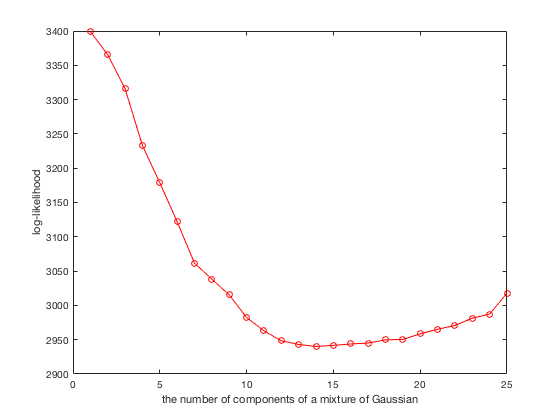
\includegraphics[scale=0.6]{fig/HW6P1_11.png}
\caption{log-likelihood as a function of the number of components of amixture of Gaussians for \textbf{data1train.dat}}
%\label{fig:HW6P1_1}
\end{figure}


fixed number of Gaussians that works well for \textbf{data1train.dat} is \textbf{14}.

\begin{figure}[h!]
\centering
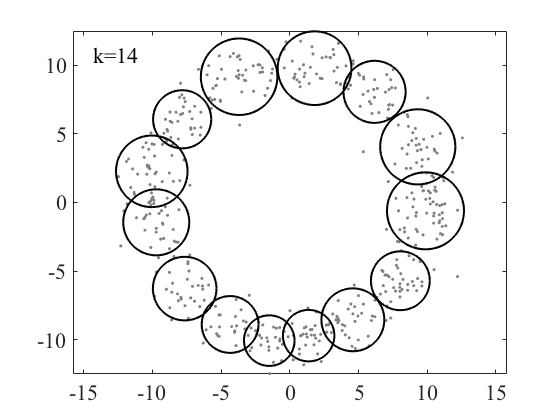
\includegraphics[scale=0.6]{fig/HW6P1_12.png}
\caption{Optimal Gaussians mixtures that work for \textbf{data1train.dat}}
%\label{fig:HW6P1_1}
\end{figure}


\newpage
List the mean, covariance and mixing weights for each mixture component.

\begin{math}
\begin{aligned}
\mbox{best mean} & \mbox{best covariance} & \mbox{best mixing weight} \\
\left( \begin{array}{c}  1.3716  \\   -9.6936
\end{array} \right) 
& \left( \begin{array}{cc}   0.8763 & 0 \\   0 & 0.8763
\end{array} \right) 
&   0.0646  \\ %1
\left( \begin{array}{c}  6.1686 \\  8.0496    
\end{array} \right)
& \left( \begin{array}{cc}   1.2756 & 0 \\   0 & 1.2756 
\end{array} \right) 
&   0.0667\\ %2
\left( \begin{array}{c}   -4.3445 \\  -8.8821 
\end{array} \right) 
& \left( \begin{array}{cc}   1.0669  & 0 \\   0 & 1.0669 
\end{array} \right) 
&   0.0471 \\ %3
\left( \begin{array}{c}  -9.7203 \\  -1.4463
\end{array} \right) 
& \left( \begin{array}{cc}   1.4420 & 0 \\   0 & 1.4420
\end{array} \right) 
&   0.0651\\ %4
\left( \begin{array}{c}  4.5894 \\  -8.5408
\end{array} \right) 
& \left( \begin{array}{cc}    1.3080 &  0 \\   0 &   1.3080
\end{array} \right) 
&   0.0724\\ %5
\left( \begin{array}{c}   9.3126 \\  4.0447 
\end{array} \right) 
& \left( \begin{array}{cc} 1.8687  & 0 \\   0 & 1.8687 
\end{array} \right) 
&   0.0747\\ %6
\left( \begin{array}{c}   -10.0447 \\  2.2659
\end{array} \right) 
& \left( \begin{array}{cc}   1.6937  & 0 \\  0   & 1.6937 
\end{array} \right) 
&   0.0809\\ %7
\left( \begin{array}{c}  -1.4953 \\  -10.0566
\end{array} \right)
& \left( \begin{array}{cc}   0.8459   & 0 \\   0 & 0.8459   
\end{array} \right) 
&   0.0510 \\ %8
\left( \begin{array}{c}   9.8751 \\  -0.6106
\end{array} \right) 
& \left( \begin{array}{cc}   1.9610 & 0 \\   0 & 1.9610 
\end{array} \right) 
&   0.1189 \\ %9
\left( \begin{array}{c} -7.6513 \\  -6.2702  
\end{array} \right) 
& \left( \begin{array}{cc}   1.3372 & 0 \\   0 & 1.3372
\end{array} \right) 
&   0.0582\\ %10
\left( \begin{array}{c}  1.8042 \\  9.7706
\end{array} \right) 
& \left( \begin{array}{cc}   1.7976 &  0 \\   0 &  1.7976
\end{array} \right) 
&   0.0787\\ %11
\left( \begin{array}{c}   8.0447 \\  -5.6998 
\end{array} \right) 
& \left( \begin{array}{cc}   1.1455  & 0 \\   0 &  1.1455 
\end{array} \right) 
&   0.0753\\ %12
\left( \begin{array}{c}   -3.6905 \\  9.1483
\end{array} \right) 
& \left( \begin{array}{cc}    1.9368 & 0 \\  0   &  1.9368
\end{array} \right) 
&   0.0844\\ %13
\left( \begin{array}{c}  -7.8340 \\  6.0516
\end{array} \right)
& \left( \begin{array}{cc}    1.1180 & 0 \\   0 &  1.1180
\end{array} \right) 
&   0.0621 %14
\end{aligned}
\end{math}


\newpage
For \textbf{data2train.dat}:


\begin{figure}[h!]
\centering
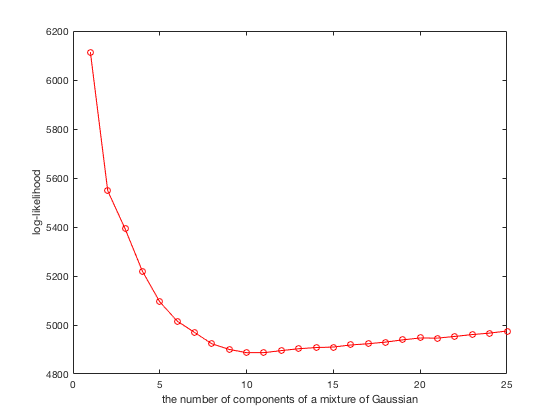
\includegraphics[scale=0.6]{fig/HW6P1_21.png}
\caption{log-likelihood as a function of the number of components of amixture of Gaussians for \textbf{data2train.dat}}
%\label{fig:HW6P1_1}
\end{figure}


fixed number of Gaussians that works well for \textbf{data1train.dat} is \textbf{10}.
\begin{figure}[h!]
\centering
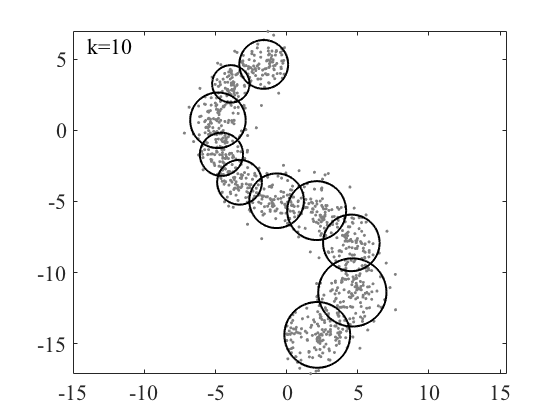
\includegraphics[scale=0.6]{fig/HW6P1_22.png}
\caption{Optimal Gaussians mixtures that work for \textbf{data2train.dat}}
%\label{fig:HW6P1_1}
\end{figure}

\newpage
List the mean, covariance and mixing weights for each mixture component.
\begin{math}
\begin{aligned}
\mbox{best mean} & \mbox{best covariance} & \mbox{best mixing weight} \\
\left( \begin{array}{c}  -4.5860 \\ -1.6871
\end{array} \right) 
& \left( \begin{array}{cc}  0.5758  &  0 \\ 0    & 0.5758
\end{array} \right) 
&  0.0793   \\ %1
\left( \begin{array}{c} 2.1473  \\  -14.3782
\end{array} \right)
& \left( \begin{array}{cc}  1.3352  & 0 \\ 0   & 1.3352
\end{array} \right) 
&  0.1471  \\ %2
\left( \begin{array}{c}   -4.8326  \\  0.7035
\end{array} \right) 
& \left( \begin{array}{cc}   0.9502 & 0  \\ 0   &  0.9502
\end{array} \right) 
&  0.1073 \\ %3
\left( \begin{array}{c}  -3.9271  \\  3.2646
\end{array} \right) 
& \left( \begin{array}{cc}   0.4316 & 0 \\  0  & 0.4316
\end{array} \right) 
&  0.0671   \\ %4
\left( \begin{array}{c} -1.6167   \\  4.6312
\end{array} \right) 
& \left( \begin{array}{cc}   0.7350   & 0  \\  0  &  0.7350 
\end{array} \right) 
&  0.1017  \\ %5
\left( \begin{array}{c}  -3.3163 \\  -3.6515
\end{array} \right) 
& \left( \begin{array}{cc}  0.6169    & 0 \\ 0   &  0.6169  
\end{array} \right) 
&   0.0778 \\ %6 
\left( \begin{array}{c} 2.1058  \\  -5.6436 
\end{array} \right)
& \left( \begin{array}{cc}  1.0695   & 0 \\  0  &  1.0695 
\end{array} \right) 
&  0.0964 \\ %7
\left( \begin{array}{c}   4.6136 \\  -11.3956
\end{array} \right) 
& \left( \begin{array}{cc}   1.4347 & 0 \\  0  & 1.4347
\end{array} \right) 
& 0.1386 \\ %8
\left( \begin{array}{c} 4.5414 \\ -7.9118 
\end{array} \right) 
& \left( \begin{array}{cc}   0.9857   & 0 \\  0  & 0.9857  
\end{array} \right) 
&  0.0924 \\ %9
\left( \begin{array}{c}  -0.7092 \\  -4.9507 
\end{array} \right) 
& \left( \begin{array}{cc}   0.9208   & 0  \\  0  & 0.9208  
\end{array} \right) 
&  0.0924  %10
\end{aligned}
\end{math}



\newpage
\section{Resampling}
Randomly generate 100 particles $x^{i}$ form some distribution $\pi$ of your choice, and 100 (positive) weights $w^{i}$. Normalize the weights such that $\sum_{i} w^{i} =1$, and the weighted samples ${x^{i},w^{i}}$ to estimate the mean $m$ of $\pi$, and denote this estimate by $\hat{m}$.

Resample the particles $x^i$ (from the weights $w^i$) using multinominal resampling, and estimate the mean from the resampled (now equally weighted) samples. Denote this estimate $\hat{m}_m$.

Repeat this for systematic resampling, and denote this estimate $\hat{m}_s$.

Repeat this for stratified resampling, and denote this estimate $\hat{m}_t$.

Repeat the items above multiple times, and report an estimate of the variance for $\hat{m}-\hat{m}_m$, $\hat{m}-\hat{m}_s$, and $\hat{m}-\hat{m}_t$ respectively, conditionally on $\hat{m}$ (that is, do not sample new particles from $\pi$, but only repeat the resampling step). Which resampling scheme appears to be the preferred one, in terms of variance?

\textbf{Solution}:

I randomly generate 100 particles $x^{i}$ using Gaussian distribution $G(0,1)$ and calculate weights $w^{i}$, normalize the weights by 
\begin{equation}
    w^{i} = \frac{w^{i}}{sum(w^{i})}
\end{equation}

Then I use the same samples and normalized weights to resample multiple times. 
The algorithms of multinomial resampling, systematic resampling and stratified resampling are in the code (see the attached code)

I repeat resample 1000 times to calculate the variance of $\hat{m}-\hat{m}_m$, $\hat{m}-\hat{m}_s$, and $\hat{m}-\hat{m}_t$.

\begin{figure}[h!]
\centering
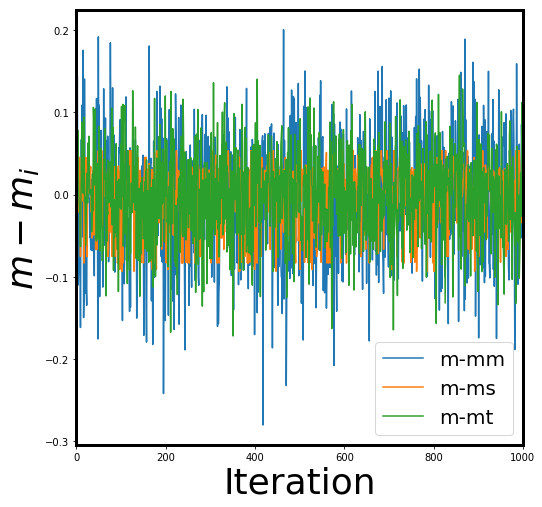
\includegraphics[scale=0.4]{fig/P5_1.png}
\caption{$\hat{m}-\hat{m}_m$, $\hat{m}-\hat{m}_s$, and $\hat{m}-\hat{m}_t$ in 1000 iterations}
%\label{fig:HW6P1_1}
\end{figure}
In this Figure 5, we find that the variance of $\hat{m}-\hat{m}_m$ is the largest. The variance of $\hat{m}-\hat{m}_s$ is smallest. 

Analytically, in our simulation, 1000 iterations.

Variance of $\hat{m}-\hat{m}_m$ is $0.005132756202771032$

Variance of $\hat{m}-\hat{m}_s$ is $0.0014684267477009338$

Variance of $\hat{m}-\hat{m}_t$ is $0.002763182508388841$

In terms of variance, systematic resampling is the preferred one.

\newpage
\section{EM algorithm}
Consider data,
\begin{equation}
    D = \left\{\left( \begin{array}{c}  1 \\  3
    \end{array} \right)
    \left( \begin{array}{c}  4 \\  5
    \end{array} \right)
    \left( \begin{array}{c}  2 \\  \star
    \end{array} \right)\right\}
\end{equation}
sampled from a two-dimensional (separable) distribution $p(x_1,x_2) = p_{x_{1}}(x_{1})p_{x_{2}}(x_{2})$ where:

\begin{equation}
p_{x_1}(x_1) = \left\{\begin{array}{rcl}
\frac{1}{\theta_1} \exp(-\frac{x_1}{\theta_1}) & \mbox{if} & x_1 \geq 0,\\ 
0  & \mbox{otherwise} ,
\end{array}\right. 
\end{equation}

and

\begin{equation}
p_{x_2}(x_2) = \left\{\begin{array}{rcl}
\frac{1}{\theta_2}  & \mbox{if} & 0 \leq x_2 \leq \theta_2,\\ 
0  & \mbox{otherwise} ,
\end{array}\right. 
\end{equation}


and $*$ in the dataset indicates a missing value.
\newline
(a) What can you infer from $\theta_2$ by looking at $D$?
\newline
\textbf{Solution}:

The  existing two pairs ($x_1$,$x_2$)  $\left( \begin{array}{c}  1 \\  3
    \end{array} \right)
    \left( \begin{array}{c}  4 \\  5
    \end{array} \right)$ mean that 
    
    for $p_{x_2}(x_2)$,$p_{3}(3) \neq 0$ and $p_{5}(5) \neq 0$.
    
    $0 \leq 3 \leq 5 \leq \theta_2$
    
Therefore, $\theta_2$  should be greater or equal to 5.
\newline
(b) Start with an initial estimate $\theta^{0}= \left( \begin{array}{c}  3 \\  6
    \end{array} \right)$ and analytically calculate $Q(\theta | \theta^{0})$. 
This is the expected joint data log-likelihood considered in class. For this problem to compute it, you effectively have to marginalize out the missing values. This is the estimate expectation step in the EM algorithm.
\newline
\textbf{Solution}:

\begin{math}
    D = \left\{\left( \begin{array}{c}  x_{11} = 1 \\  x_{12} = 13
    \end{array} \right)
    \left( \begin{array}{c}  x_{21} =  4 \\ x_{22} = 5
    \end{array} \right)
    \left( \begin{array}{c} x_{31} = 2 \\  x_{32} = \star
    \end{array} \right)\right\}
\end{math}

$\theta^{0}= \left( \begin{array}{c}  \theta_1^{0} = 3 \\ \theta_2^{0} =  6
    \end{array} \right) = (\theta_1^{0},\theta_2^{0})$ 
    
$\theta= \left( \begin{array}{c}  \theta_1  \\ \theta_2
    \end{array} \right) = (\theta_1,\theta_2)$

\begin{equation}
\begin{aligned}
    p(x_1,x_2,\theta) & = p_{x_1}(x_1 | \theta) p_{x_2}(x_2 | \theta) \\
                      & = \left\{\begin{array}{rcl}
\frac{1}{\theta_1} \exp(-\frac{x_1}{\theta_1}) \frac{1}{\theta_2}  & \mbox{if} & x_1 \geq 0  \&  0 \leq x_2 \leq \theta_2,\\ 
0  & \mbox{otherwise} ,
\end{array}\right. 
\end{aligned}
\end{equation}

Then we need to use the expected joint data log-likelihood $Q(\theta | \theta^{0})$.

\begin{equation}
\begin{aligned}
& Q(\theta | \theta^{0})  = E_{x_{32}}[\ln{p(x_v,x_h,\theta)} | \mathcal{D},\theta^{0}] \\
& = \int_{-\infty}^{\infty} [\ln{p(x_{11},x_{12} | \theta)} + \ln{p(x_{21},x_{22} | \theta)}+ \ln{p(x_{31},x_{32} | \theta)}] p(x_{32} |x_{31},\theta^{0}) dx_{32} \\
& = \ln{p(x_{11},x_{12} | \theta)} + \ln{p(x_{21},x_{22} | \theta)} + \int_{-\infty}^{\infty} [ \ln{p(x_{31},x_{32} | \theta)}] \frac{p(x_{31},x_{32}|\theta^{0})}{\int_{-\infty}^{\infty} p(x_{31}, x_{32}^{'} |\theta^{0}) dx_{32}^{'} } dx_{32}
\end{aligned}
\end{equation}

\begin{equation}
\begin{aligned}
\ln{p(x_{11},x_{12} | \theta)} + \ln{p(x_{21},x_{22} | \theta)} & = \ln(\frac{1}{\theta_1 \theta_2}e^{-\frac{x_{11}}{\theta_1}}) +\ln(\frac{1}{\theta_1 \theta_2}e^{-\frac{x_{21}}{\theta_1}})  \\
& =\ln(\frac{1}{\theta_1 \theta_2}e^{-\frac{1}{\theta_1}}) +\ln(\frac{1}{\theta_1 \theta_2}e^{-\frac{4}{\theta_1}}) \\
& = -2 \ln{\theta_1 \theta_2} -\frac{5}{\theta_1}
\end{aligned}
\end{equation}

\begin{equation}
p(x_{31}=2,x_{32} | \theta^{0}) = p_{x_{31}}(x_{31}=2|\theta^{0}) p_{x_{32}}(x_{32}|\theta^{0})    
\end{equation}

\begin{equation}
\int_{-\infty}^{\infty} p(x_{31}=2, x_{32}^{'} |\theta^{0}) dx_{32}^{'} = p_{x_{31}}(x_{31}=2|\theta^{0})  
\end{equation}

\begin{equation}
\begin{aligned}
 \int_{-\infty}^{\infty} [ \ln{p(x_{31},x_{32} | \theta)}] \frac{p(x_{31},x_{32}|\theta^{0})}{\int_{-\infty}^{\infty} p(x_{31}, x_{32}^{'} |\theta^{0}) dx_{32}^{'} } dx_{32} = \int_{-\infty}^{\infty} [ \ln{p(x_{31},x_{32} | \theta)}] p_{x_{32}}(x_{32}|\theta^{0}) dx_{32}
\end{aligned}
\end{equation}

$[ \ln{p(x_{31},x_{32} | \theta)}] p_{x_{32}}(x_{32}|\theta^{0}) \neq 0$ if $ 0 \leq x_{32} \leq \min(\theta_2,  \theta_{2}^{0}=6) = \min(\theta_2,  6) $

\begin{equation}
\begin{aligned}
 \int_{-\infty}^{\infty} [ \ln{p(x_{31},x_{32} | \theta)}] p_{x_{32}}(x_{32}|\theta^{0}) dx_{32} = \int_{0}^{\min(\theta_2,  6)} ( -\ln{\theta_1 \theta_2} -\frac{2}{\theta_1}) (\frac{1}{6}) dx_{32}
\end{aligned}
\end{equation}

\begin{equation}
\begin{aligned}
 \mbox{for }   & 5 \leq \theta_2 <6, \theta_2=\min(\theta_2,  6) \\
& \int_{-\infty}^{\infty} [ \ln{p(x_{31},x_{32} | \theta)}] p_{x_{32}}(x_{32}|\theta^{0}) dx_{32} \\
& = \int_{0}^{\theta_2} ( -\ln{\theta_1 \theta_2} -\frac{2}{\theta_1}) (\frac{1}{6}) dx_{32} \\
& = \frac{\theta_2}{6}(-\ln{\theta_1 \theta_2} -\frac{2}{\theta_1})
\end{aligned}
\end{equation}

\begin{equation}
\begin{aligned}
 \mbox{for }   & 6 \leq \theta_2 , 6=\min(\theta_2,  6) \\
& \int_{-\infty}^{\infty} [ \ln{p(x_{31},x_{32} | \theta)}] p_{x_{32}}(x_{32}|\theta^{0}) dx_{32} \\
& = \int_{0}^{6} ( -\ln{\theta_1 \theta_2} -\frac{2}{\theta_1}) (\frac{1}{6}) dx_{32} \\
& = (-\ln{\theta_1 \theta_2} -\frac{2}{\theta_1})
\end{aligned}
\end{equation}


Therefore, combine (11)(16)(17).
\begin{equation}
\begin{aligned}
\mbox{for }   & 5 \leq \theta_2 <6 \\
& Q(\theta | \theta^{0})  = -2 \ln{\theta_1 \theta_2} -\frac{5}{\theta_1} + \frac{\theta_2}{6}(-\ln{\theta_1 \theta_2} -\frac{2}{\theta_1})    = -(2+\frac{\theta_2}{6})\ln{\theta_1 \theta_2} -(5+\frac{\theta_2}{3}) \frac{1}{\theta_1} \\
 \mbox{for }   & 6 \leq \theta_2  \\
& Q(\theta | \theta^{0})  = -2 \ln{\theta_1 \theta_2} -\frac{5}{\theta_1} +  (-\ln{\theta_1 \theta_2} -\frac{2}{\theta_1}) 
= -3\ln{\theta_1 \theta_2} -\frac{7}{\theta_1}
\end{aligned}
\end{equation}

(c) Find the $\theta$ that maximizes your  $Q(\theta | \theta^{0})$. This is the maximization step of the EM algorithm.
\newline
\textbf{Solution}:

\textbf{M} step: solving $ \bigtriangledown Q(\theta | \theta^{0})= 0 $ or get the maximization of 
$Q(\theta | \theta^{0})$

We have the boundary conditions for $\theta_2$, so we start from $\theta_2$.

\begin{equation}
    \frac{\partial Q(\theta | \theta^{0})}{ \partial \theta_2 }
\end{equation}

\begin{equation}
\begin{aligned}
\mbox{for }   & 5 \leq \theta_2 <6 \\
& \frac{\partial Q(\theta | \theta^{0})}{ \partial \theta_2 } = -\frac{\ln \theta_1}{6}-\frac{1}{3\theta_1} -\frac{2}{\theta_2}- \frac{\ln \theta_2}{6}  -\frac{1}{6} \\ 
& = F(\theta_1)+G(\theta_2)-\frac{1}{6} 
\end{aligned}
\end{equation}

\begin{equation}
\begin{aligned}
F(\theta_1) = -\frac{\ln \theta_1}{6}-\frac{1}{3\theta_1}
\end{aligned}
\end{equation}

\begin{equation}
\begin{aligned}
\frac{\partial F(\theta_1)}{ \partial \theta_1} = \frac{1}{6} (\frac{1}{\theta_1}-\frac{2}{(\theta_{1})^{2}}) = 0  \rightarrow \theta_1 = 2 
\end{aligned}
\end{equation}

\begin{equation}
\begin{aligned}
F(\theta_1) \leq F(2) = -\frac{1}{6}(\ln2 +1) <0
\end{aligned}
\end{equation}

\begin{equation}
\begin{aligned}
G(\theta_2) = -\frac{2}{\theta_2}- \frac{\ln \theta_2}{6} < 0 & \mbox{for } & 5 \leq \theta_2 <6
\end{aligned}
\end{equation}

Therefore,

\begin{equation}
\begin{aligned}
\mbox{for }   & 5 \leq \theta_2 <6 \\
& \frac{\partial Q(\theta | \theta^{0})}{ \partial \theta_2 } < 0
\end{aligned}
\end{equation}

\begin{equation}
\begin{aligned}
\mbox{for }   & 6 \leq \theta_2  \\
& \frac{\partial Q(\theta | \theta^{0})}{ \partial \theta_2 } = -\frac{3}{\theta_2} < 0
\end{aligned}
\end{equation}

And $Q(\theta | \theta^{0})$ is continuous at $\theta=6$. Therefore, for $5 \leq \theta_2 <6$ and $6 \leq \theta_2 $, $Q(\theta | \theta^{0})$ is monotonically continuous decreasing. 

When $\theta_2 = 5$, $Q(\theta | \theta^{0})$ gets the largest value $Q(\theta_1,\theta_2 = 5 | \theta^{0})$ . Then we fix $\theta_2 = 5$ and solve $\theta_1$. 

\begin{equation}
\begin{aligned}
Q(\theta_1,\theta_2 = 5 | \theta^{0}) = -(\frac{17}{6})\ln{5\theta_1} -(\frac{20}{3}) \frac{1}{\theta_1}
\end{aligned}
\end{equation}

$\theta_1 > 0$

\begin{equation}
\begin{aligned}
& \frac{\partial Q(\theta_1,\theta_2 = 5 | \theta^{0})}{ \partial \theta_1 } = -(\frac{17}{6})\frac{1}{\theta_1} + (\frac{20}{3}) \frac{1}{(\theta_1)^2} = 0 \rightarrow \theta_1 = \frac{40}{17}
\end{aligned}
\end{equation}

\begin{equation}
\begin{aligned}
& \frac{\partial Q(\theta_1,\theta_2 = 5 | \theta^{0})}{ \partial \theta_1 } >0 & \mbox{if } & 0<\theta_1 < \frac{40}{17} \\
& \frac{\partial Q(\theta_1,\theta_2 = 5 | \theta^{0})}{ \partial \theta_1 } <0 & \mbox{if } & \frac{40}{17} < \theta_1 
\end{aligned}
\end{equation}

$Q(\theta_1,\theta_2 = 5 | \theta^{0})$ gets the largest value when $\theta_1 = \frac{40}{17}$.

In conclusion, the $\theta= \left( \begin{array}{c}  \theta_1 \\  \theta_2
    \end{array} \right) =\left( \begin{array}{c}  \frac{40}{17} \\  5
    \end{array} \right) $ maximizes $Q(\theta | \theta^{0})$. 

%\bibliographystyle{plain}
%\bibliography{references}
\end{document}
